%%%%%%%%%%%%%%%%%%%%%%%%%%%%%%%%%%%%%%%%%%%%%%%%%%%%%%%%%%%%%%%%%%%%%%%%%%%%%%
%%%%%%%%%%%%%%%%%%%%%%%%%%%%%%%%%%%%%%%%%%%%%%%%%%%%%%%%%%%%%%%%%%%%%%%%%%%%%%
%%
%% Dokumentacia k semestralnemu projektu z PRL2
%%
%%%%%%%%%%%%%%%%%%%%%%%%%%%%%%%%%%%%%%%%%%%%%%%%%%%%%%%%%%%%%%%%%%%%%%%%%%%%%%
%%%%%%%%%%%%%%%%%%%%%%%%%%%%%%%%%%%%%%%%%%%%%%%%%%%%%%%%%%%%%%%%%%%%%%%%%%%%%%
\documentclass[11pt,a4paper,titlepage,final]{article}

% cestina a fonty
\usepackage[czech]{babel}
\usepackage[T1]{fontenc}
\usepackage[utf8]{inputenc}
% balicky pro odkazy
\usepackage[bookmarksopen,colorlinks,plainpages=false,urlcolor=blue,unicode]{hyperref}
\usepackage{url}
% obrazky
\usepackage[dvipdf]{graphicx}
% velikost stranky
\usepackage[top=3.5cm, left=2.5cm, text={17cm, 24cm}, ignorefoot]{geometry}
\usepackage{fancyhdr}

\begin{document}
\raggedright\large{\textbf{Projekt z predmetu PRL Martin Maga (xmagam00) \\Carry Look Ahead Parallel Binary Adder}}

\section{Teoretické rozobratie algoritmu}
Algoritmus je postavený na myšlienke sčítania 2 binárnych čísel pomocou binárnych sčítačiek (reprezentovanými procesormi), ktoré na vstupe majú i-tý bit z daného binárneho čísla a prenos. Jednotlivé sčítačky generajú pri sčitaní i-tého bitu prenos $c_i$, ktorý sa prenáša do ďalšej sčítačky. Pri tomto algoritme je potreba ešte pred samostatným výpočtom vyriešiť všetky bity prenosu $c_(n-1)$ \ldots $c_0$, aby sme mohli priamo paralelne spočítať $z_i$ = $x_i$ + $y_i$ + $c_i$.


\section{Časová zložitosť}
Časová zložitosť tohto algoritmu je priamo ovplyvnená tým, že pred každým výpočtom je nutné vyrieši všetky bity prenosu $c_(n-1)$ \ldots $c_0$. Všetky bitu prenosu dostanme presne po log n krokoch. Samostný výpočet následne zabere presne 1 krok. Celková časová zložitosť tohto algoritmu je: \textbf{t(n) = log n + 1}.

\section{Priestorová zložitosť}
V tomto algoritme používame binárne sčítačky, keďže celý výpočet je paralelizovaný každú binárnu sčítačk reprezentuje 1 procesor. Celkovo pre n-bitové číslo potrebuje n procesorov, pričom každú má na vstupe práve 1 bit z každého číslo a prenos z predchádzajúceho výpočtu z binárnej sčítačky. Priestorová zložitosť je: \textbx{p(n) = n}


\section{Celková cena algoritmu}
Celková cena algoritmu je: c(n) = p(n) * t(n). Pre náš algoritmus dostávame hodnotu: c(n) = (log n + 1)*n = $n * log n$ (pri zanedbaní nejakých premenných). Celková cena riešenia je semilogaritická, je ešte optimálne pre paralelné riešenie.

\section{Implementácia}
Pri implementácií algoritmu Carry Look Ahead Parallel Binary Adder bola použivá knižnica OpenMPI spolu s jazykom C+. Táto knižnica umožňuje implementáciu algoritmov paralelne, pričom vytvára procesory (similuje ich), ktoré komunikujú prostredníctvom správ. Program clapba.cpp po preložení paralelne vytvorí N procesorov podľa 1. parametru v skripte test.sh, ktorý zároveň vytvorý 2 binárne čísla  v súbore numbers. Každý procesor si pri vytvorení uchová svoje jedinečné číslo, s ktorým ďalej pracuje. Celý algoritmus je spustení z 1. procesora, teda z procesora s $my_id$ s hodnotou 0. Tento procesor načíta vstupný súbor "numbers" a jednotlivé čísla následne prepošle ďalšim procesorom. 

Celý algoritmus 
Celý algoritmus pokračuje obdržaním hodnôt od koreňa stromu a jej uložením do pomocnej premennej.Následne sa realizuje nekonečný cyklus. V tomto cykle sa postupne realizuje nasledovné. Pre každý ne-koreňový a zároveň listový procesor sa zistí id procesory jeho rodiča(v závislosti od jeho aktuálneho $my_id$). Ten pošle hodnotu svojho čísla rodičovi a prijme hodnotu od rodiča. Pokiaľ nejaký uzol dostane od rodiča hodnotu "-1", znamená,  že svoju uloženú hodnotu poslal už svojmu rodičovi a zároveň táto hodnota bola zároveň menšia ako hodnota jeho brata a teda môže svoju činnosť skončiť, keďže je listový. Preto sa aj procesor následne ukončí. Treba podotknúť akým spôsobom sa pracuje s premennou $"my_id"$, ktorá obsahuje jedinečné číslo pre každý procesor. Hodnota 0 predstavuje koreň stromu, hodnoty 1 - ((počet zadaných procesorov + 1) / 2) - 2 sú hodnoty nelistových procesorov a hodnoty ((počet zadaných procesorov + 1) / 2) - 1 až počet zadaných procesorov predstavuje listové procestory.

Pre každý nelistový procesor sa zistí, od ktorých procesorov (potomkov) má získať hodnoty. Ten získa obe hodnoty a menšiu z nich si uloží a prepošle svojmu rodičovu (opäť k výpočtu rodiča použije hodnotu $my_id$). Väčšiu hodnotu pošle späť svojmu potomkovi, od ktorého ju održal a potomkovi, od ktorého získal menšiu hodnotu pošle hodnotu "-1" na ukončenie.  Tento proces sa neustále opakuje pokiaľ procesor nie je ukončený, tj neobdržal hodnota -1 od svojho rodiča. Ako postupne hodnoty postupujú až dosiahnu koreň. Ten postupne vypisuje hodnoty, ktoré obdržal na výstup a pošle sa hodnota "-1" nelistovému procesoru, od ktorého obdržal menšiu hodnotu a druhému potomkovi pošle hodnotu späť. Až nakoniec sám obdŕži hodnotu -1 => všetky ostatné procesory sú ukončené a sám sa ukončí.


\section{Komunikačný protokol}
Na nasledujúcom obrázku je zobrazený komunikačný protokol:
 \begin{figure}[h]

\begin{center}
\scalebox{0.15}{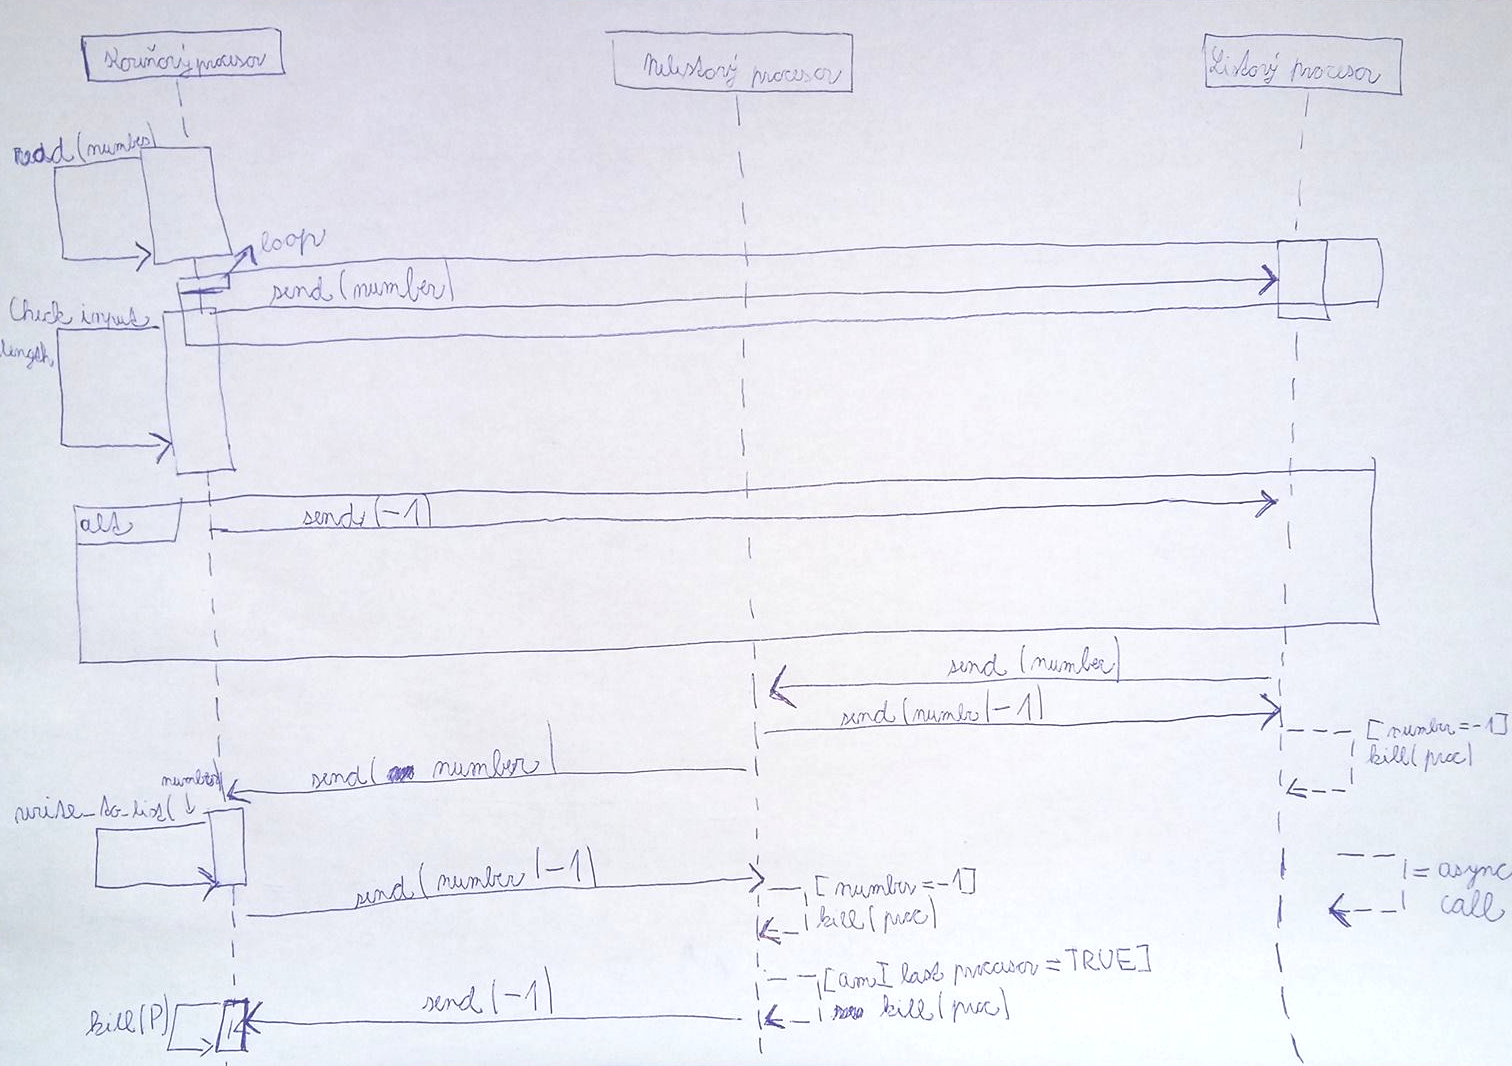
\includegraphics{img/diagram.eps}}
\caption{Sekvenčí diagram popísujúci komunikáciu}
\end{center}

\end{figure}


\section{Experimenty}
V tejto kapitole sme overovali časovú zložitosť, ktorá je približne logaritmická. Z tohto môžme predpokladať, že výsledný graf bude mať tvar logaritmickej krivky. Pre overenie sme vykonali experiment nasledovne: Ako vstup sme postupne spúštali skript test.sh nasledovne: 1.beh test.sh 1, 2. beh test.sh 2 ,3.beh test.sh 3, 4.beh test.sh 4, 5.beh test.sh 5, 6.beh test.sh 6, 7.beh test.sh 7, 8.beh test.sh 8, 9.beh test.sh 9, 10.beh test.sh 10, 11.beh test.sh 11, 12.beh test.sh 12, 13.beh test.sh 13, 14.beh test.sh 14, 15.beh test.sh 15, 16.beh test.sh 16, 17.beh test.sh 17, 18.beh test.sh 18, 19.beh test.sh 19, 20.beh test.sh 20.

Algoritmus sme spúštali na serveri merlin(Linux merlin.fit.vutbr.cz 3.12.56 $x86\_64$ GNU/Linux). Pre správnosť výsledkov sme každú konfiguráciu spustili 100x a výsledný čas som spriemeroval. Treba spomenúť, že nebolo možné overiť riešenie pre väčší počet hodnôt, keďže server merlin nedovoluje spustiť program s väčším počtu procesorov.

Z implementačného hľadiska treba podotknúť, že meranie je realizované funkcou $"MPI_Wtime()"$, ktorá vracia počet sekúnd. Tento funkcia sa volá na začiatku a na konci pre koreňový procesor.
 \begin{figure}[h]

\begin{center}
\scalebox{0.5}{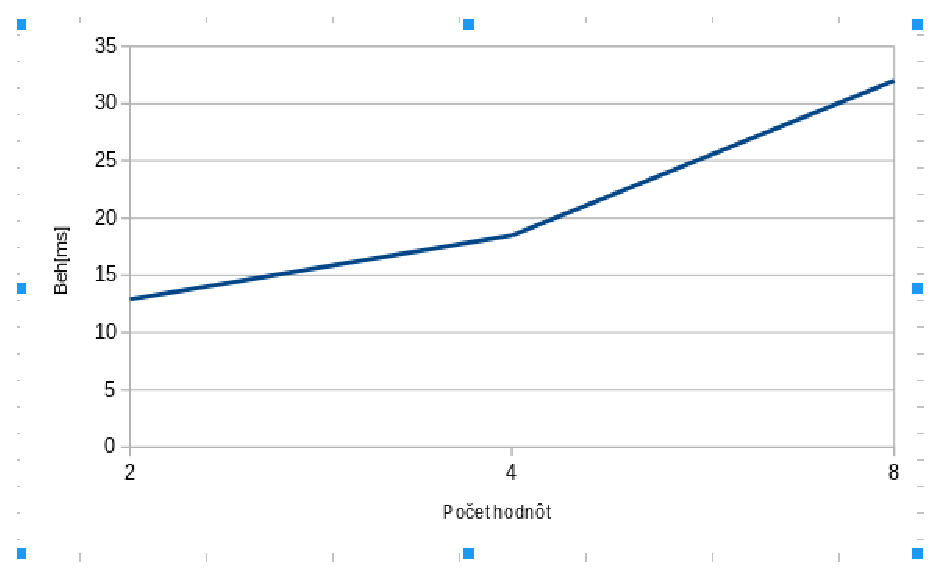
\includegraphics{img/mes.eps}}
\caption{Graf časovej závislosti počtu vstupných hodnôt a behu programu v ms}
\end{center}

\end{figure}

\section{Záver}
Implementovali sme algoritmus Carry Look Ahead Parallel Binary Adder s knižnicou OpenMPI. Rovnako sme odvodili teoretickú časovú, priestorovú a celkovú zložitosť algoritmu, ktorú sme experimentom aj potvrdili.
\end{document}



